\section{马踏棋盘}

\subsection{算法介绍}

\subsubsection{实验具体要求}

\begin{figure}[H]
  \flushleft
  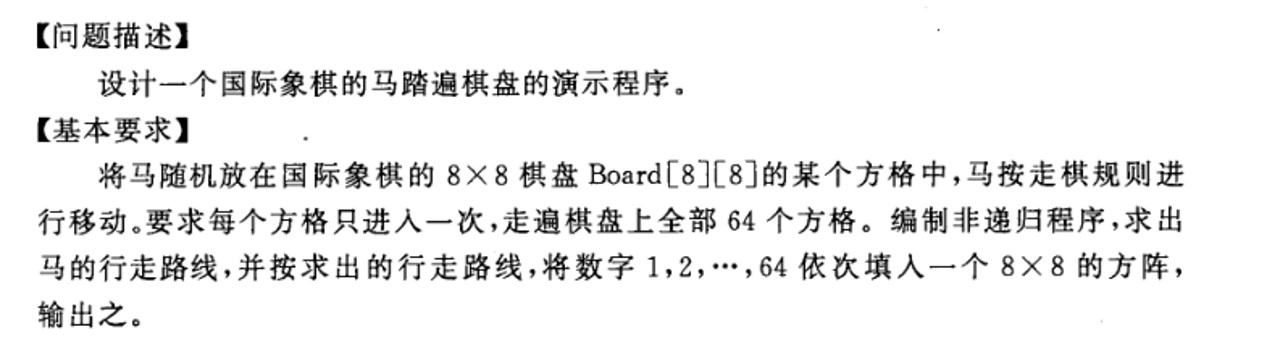
\includegraphics[width=15cm]{fig/KTP1.jpg}
  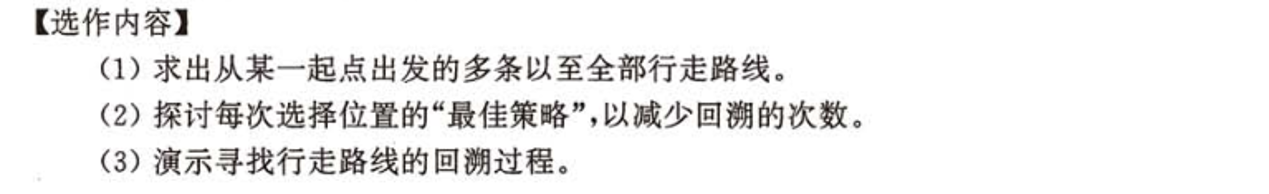
\includegraphics[width=15cm]{fig/KTP2.png}
\end{figure}

\noindent
需要写出一个非递归的程序使马在以“日”字行走的过程中遍历一个$8 \times 8$棋盘上的每一个点,下面讲解具体实现。

\vspace{1ex}

\subsubsection{关键数据结构说明}

% \begin{figure}[H]
%   \centering
%   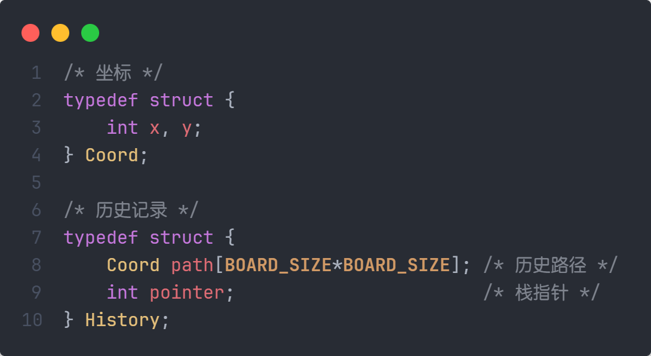
\includegraphics[width=10cm]{fig/KTP3.png}
%   \caption{KTP数据结构}
% \end{figure}

    /* 坐标 */
    typedef struct {
        int x, y;
        int block[8]; /* 下一步不可走的方向 */
    } Coord;

    /* 历史记录 */
    typedef struct {
        Coord path[BOARD_SIZE*BOARD_SIZE]; /* 历史路径 */
        int pointer;                       /* 栈指针   */
    } History;
% \end{lstlisting}

\noindent
其中{\tt Coord}用来记录坐标,包括两个成员{\tt x}和{\tt y};{\tt History}用来记录到目前位置的所有历史记录,从第$0$步(初始坐标)开始计数,有两个成员:{\tt path}数组(历史路径)和{\tt pointer}(栈指针),本质上是一个栈。

\vspace{1ex}

\subsubsection{贪心算法}

\noindent
使用贪心算法,旨在求出马所在这个格子周围八个方向分别有几个下一步,将这$8$个具体的数值存放在{\tt next[8]}数组中。每次优先选择下一步最少且合法(在棋盘内的空格子)的方向对应的点进行入栈{\tt push()}操作。

\vspace{1ex}

\noindent
入栈操作{\tt push()}与教材相同,都是通过指针的移动实现。

% \begin{figure}[H]
%   \centering
%   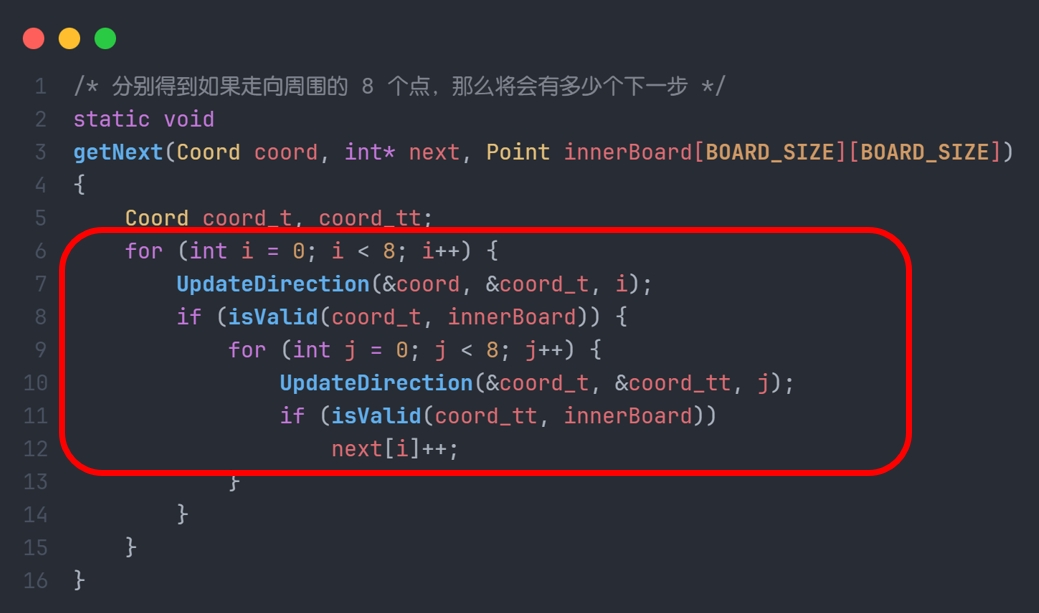
\includegraphics[width=10cm]{fig/KTP5.png}
%   \caption{实现getnext()操作}
% \end{figure}

\begin{lstlisting}[language=C, caption={实现{\tt getnext()}操作}]
    /* 分别得到如果走向周围的 8 个点,那么将会有多少个下一步 */
    static void
    getNext(Coord coord, int* next, Point innerBoard[BOARD_SIZE][BOARD_SIZE])
    {
        Coord coord_t, coord_tt;
        for (int i = 0; i < 8; i++) {
            UpdateDirection(&coord, &coord_t, i);
            if (isValid(coord_t, innerBoard)) {
                for (int j = 0; j < 8; j++) {
                    UpdateDirection(&coord_t, &coord_tt, j);
                    if (isValid(coord_tt, innerBoard))
                        next[i]++;
                }
            }
        }
    }
\end{lstlisting}

\vspace{1ex}

\noindent
利用{\tt for}循环,求出每个方向周围都有几个合法的点可以走,存在{\tt next[8]}中。

% \begin{figure}[H]
%   \centering
%   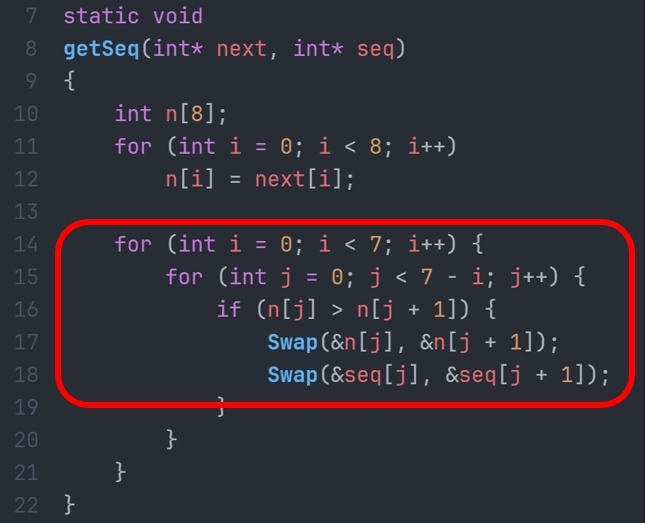
\includegraphics[width=10cm]{fig/KTP6.png}
%   \caption{对next中值实现从小到大的排序操作}
% \end{figure}

\begin{lstlisting}[language=C, caption={对{\tt next}中值实现从小到大的排序操作}]
    /*
    ** 由贪心算法,我们要给 next 数组进行非递减排序
    ** 并将具体方向对应地编号写到 seq 数组中
    ** 例如 next[3] = {5, 8, 2}
    ** 那么 seq [3] = {2, 0, 1}
    */
    static void
    getSeq(int* next, int* seq)
    {
        int n[8];
        for (int i = 0; i < 8; i++)
            n[i] = next[i];

        for (int i = 0; i < 7; i++) {
            for (int j = 0; j < 7 - i; j++) {
                if (n[j] > n[j + 1]) {
                    Swap(&n[j], &n[j + 1]);
                    Swap(&seq[j], &seq[j + 1]);
                }
            }
        }
    }
\end{lstlisting}

\vspace{1ex}

\noindent
排在前面的即是优先级高的某一个方向,注意{\tt next}为$0$的会排在前面,但是不会产生影响,因为在贪心算法总体实现的{\tt getNextStep()}中该方向会被{\tt if(isValid)}筛出去。

% \begin{figure}[H]
%   \centering
%   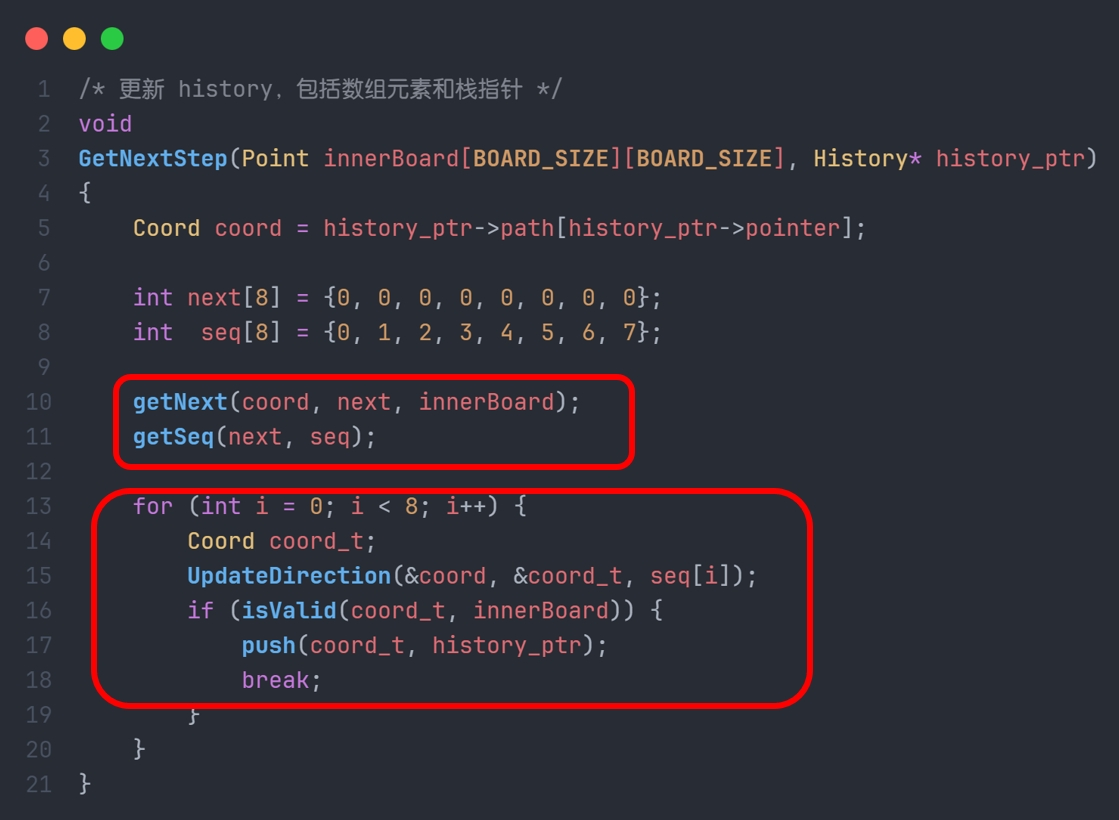
\includegraphics[width=10cm]{fig/KTP4.png}
%   \caption{贪心算法的总实现}
% \end{figure}

\begin{lstlisting}[language=C, caption={贪心算法的总实现}]
    /* 更新 history,包括数组元素和栈指针 */
    void
    GetNextStep(Point innerBoard[BOARD_SIZE][BOARD_SIZE], History* history_ptr)
    {
        Coord coord = history_ptr->path[history_ptr->pointer];

        int next[8] = {0, 0, 0, 0, 0, 0, 0, 0};
        int  seq[8] = {0, 1, 2, 3, 4, 5, 6, 7};

        getNext(coord, next, innerBoard);
        getSeq(next, seq);

        for (int i = 0; i < 8; i++) {
            Coord coord_t;
            UpdateDirection(&coord, &coord_t, seq[i]);
            if (isValid(coord_t, innerBoard)) {
                push(coord_t, history_ptr);
                break;
            }
        }
    }
\end{lstlisting}

\subsection{棋盘设计说明}

棋盘使用{\tt UTF-8}字符实现,马的位置用{\tt UTF-8}字符“马(国际象棋)”表示,棋盘也用{\tt UTF-8}字符“田”表示,空白处用空格表示。不同类型字符用不同颜色表示,以区分。

此外,为了方便观察,我们在棋盘边上标出了每个格子的坐标,在顶部显示当前马的坐标,以及当前步数,以便于观察马的移动路径。

\subsection{时空性能分析}

\subsubsection{时间复杂度}

因为无论棋盘大小如何,遍历的时候都是只有$8$个不同的方向,所以对于单独一步的判断,均只需要$64$步,时间复杂度为$\mathcal{O}(1) $,对于$n \times n$大小的棋盘 ,所需时间复杂度为$\mathcal{O}(n^2)$。


\vspace{1ex}

\subsubsection{空间复杂度}

需要用$\mathcal{O}(n^2)$的栈来记录历史路径,贪心算法所占用空间可复用,所以总空间复杂度为$\mathcal{O}(n^2)$。


\vspace{1ex}

\subsection{实例演示及优越性分析}

\subsubsection{成果展示}

\begin{figure}[H]
    \centering
    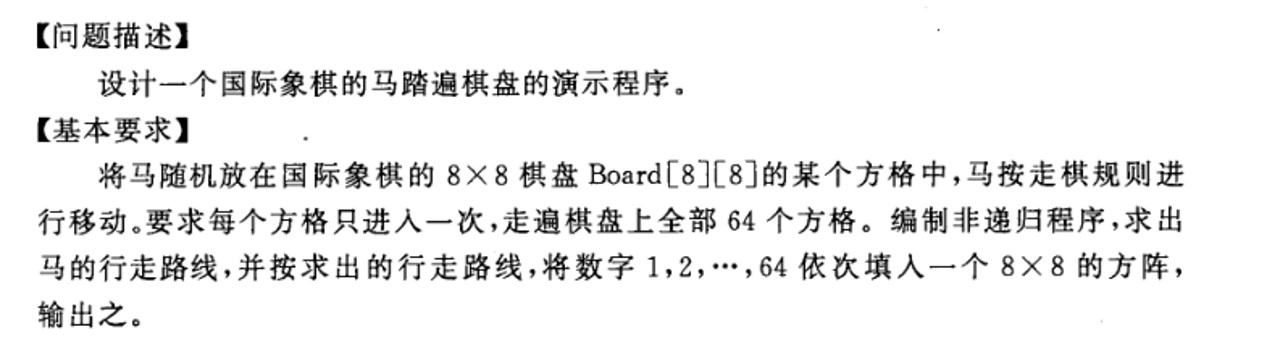
\includegraphics[width=15cm]{fig/KTP1.png}
    \caption{标题界面}
\end{figure}

\begin{figure}[H]
    \centering
    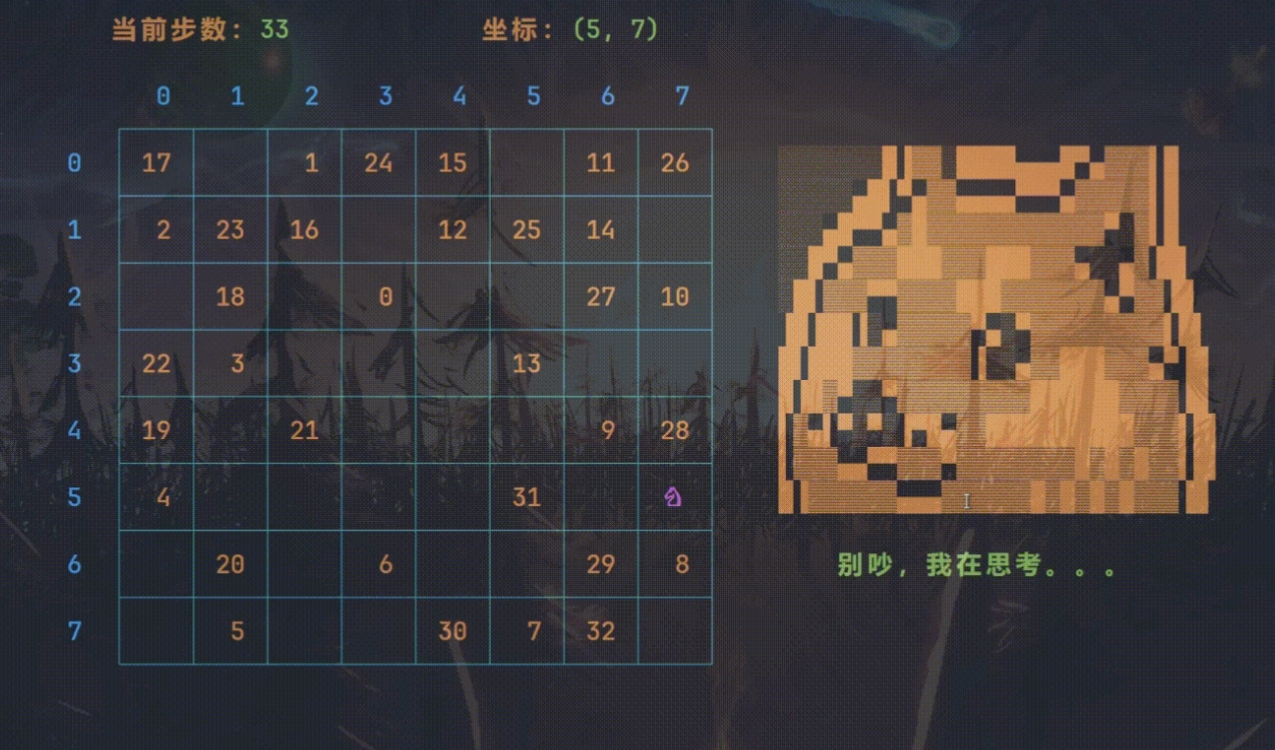
\includegraphics[width=15cm]{fig/KTP7.png}
    \caption{动画展示中某一时刻的截图}
\end{figure}

\vspace{1ex}

\subsubsection{KTP完成度总结}

由于$8 \times 8$棋盘的对称性,将棋盘以“田”字四等分,我们只需要令左上角那一个$4 \times 4$小块的一个上三角区中所有点作为初始点进行验证,就可以得到是否以棋盘上$64$个点中任意一点作为起始点,这个马踏棋盘的过程都有解。

通过我们的验证得知,这个答案是肯定的,这也说明了通过贪心算法,我们可以找到最优路径(不需要悔棋),既实现了选做2的要求,又在某种程度上实现了选做3。

\vspace{1ex}

\subsubsection{亮点总结}

\begin{enumerate}
    \item 单步打印,可以清晰看到马走完整个棋盘的全过程,且每一步停留的延时可以自己调节
    \item 健壮性:对于预期范围之外的输入能正确检测并进行处理,不会出现死循环或者异常退出的情况
    \item 通过纯{\tt C}语言实现,在命令行终端打印结果,同时支持{\tt Linux}和{\tt Windows}环境,
    资源占用小,兼容性强
    \item 可以通过修改宏改变棋盘大小和打印策略(延迟时间,是否手动跟进下一步等)
    \item 虽然在终端打印,但并不简陋,包含颜色丰富的标题界面和棋盘,用{\tt UTF-8}字符实现棋盘和马的打印
\end{enumerate}
